\date{}
\title{}
\date{}
\begin{document}
\begin{frame}
    \titlepage
\end{frame}


\makeatletter
\newenvironment<>{btHighlight}[1][]
{\begin{onlyenv}#2\begingroup\tikzset{bt@Highlight@par/.style={#1}}\begin{lrbox}{\@tempboxa}}
{\end{lrbox}\bt@HL@box[bt@Highlight@par]{\@tempboxa}\endgroup\end{onlyenv}}

\newcommand<>\btHL[1][]{%
  \only#2{\begin{btHighlight}[#1]\bgroup\aftergroup\bt@HL@endenv}%
}
\def\bt@HL@endenv{%
  \end{btHighlight}%   
  \egroup %
}
\tikzset{
    btHLbox/.style={
        fill=red!30,outer sep=0pt,inner xsep=1pt, inner ysep=0pt, rounded corners=3pt
    },
}
\newcommand{\bt@HL@box}[2][]{%
  \tikz[#1]{%
    \pgfpathrectangle{\pgfpoint{1pt}{0pt}}{\pgfpoint{\wd #2}{\ht #2}}%
    \pgfusepath{use as bounding box}%
    \node[text width={},draw=none,anchor=base west, btHLbox, minimum height=\ht\strutbox+1pt,#1]{\raisebox{1pt}{\strut}\strut\usebox{#2}};
  }%
}

\lst@CCPutMacro
    \lst@ProcessOther {"2A}{%
      \lst@ttfamily 
         {\raisebox{2pt}{*}}% used with ttfamily
         {\raisebox{2pt}{*}}}% used with other fonts
    \@empty\z@\@empty

\lstdefinelanguage
   [x8664gas]{Assembler}     % add a "x64" dialect of Assembler
   [x86masm]{Assembler} % based on the "x86masm" dialect
   % with these extra keywords:
   {morekeywords={CDQE,CQO,CMPSQ,CMPXCHG16B,JRCXZ,LODSQ,MOVSXD,%
                  POPFQ,PUSHFQ,SCASQ,STOSQ,IRETQ,RDTSCP,SWAPGS,.TEXT,.STRING,.ASCIZ,%
                  BEQ,LW,SW,LB,SB,ADDIU,J,BEQZ,BNEZ,BNE,%
                  MOVUPD,MULPD,MOVSD,MULSD,%
                  SHLADD,MOV,CMP.LT,TBIT.NZ,BR.RET.SPTK.MANY,%
                  ADDQ,POPQ,PUSHQ,RRMOVQ,MRMOVQ,RMMOVQ,IRMOVQ,%
                  <-,LL,SC,ADDI,ADDL,VMOVDQA,ADDQ,CMPL,JB,JBE,MOVL,CLTQ,%
                  MOVW,PUSHW,MOV,ADD,SUB,INT,PUSH,MOV,ADD,REP,MOVSB,%
                  TESTQ,CMPQ,MOVL,MOVQ,ADDQ,JMPQ,XORQ,%
                  LEAQ,LEAL,LEA,RETQ,RET,POPL,POPW,PUSHL,PUSHW,%
                  LEAW,%
                  SUBQ,SYSCALL,.ASCII,CALLQ,MOVSLQ,JMP,ANDQ,SHRQ,MOVB,INCQ,TESTL,XORL,%
                  SHRL,LEAL,SARL,SUBL,IMULL,IMULQ,MOVDQU,PADDD,XORL,%
                  MOVZBL,MOVZB,SHRB,SRAL,SHRL,ANDL,%
                  CMOVNS,SRAL,SRAQ,MOVZBW,MOVZBQ,%
                  PADDW,PADDQ,MODUPS,MOVAPD,%
                  MOVL,RET,.GLOBL,%
		  PAUSE,LFENCE,JMP,%
                  },
    deletekeywords={eax,ebx,sp,si,cx,di,ds,cs,es,fs,dx,ax,bx,al,esi,ebp,ecx,rip,eip,edx,edi,rdi,esp},
    deletekeywords=[2]{size},
    alsoletter={\%},
    alsoother={()},
    emphstyle={\color{violet!50!black}},
    emph={\%rax,\%rbx,\%rcx,\%rdx,\%r8,\%r9,\%r10,\%r11,\%r12,\%r13,\%r14,\%r15,\%eax,\%ebx,\%sp,\%si,\%cx,\%di,\%ds,\%cs,\%es,\%fs,\%dx,\%ax,\%bx,\%al,\%esi,\%ebp,\%ecx,\%rip,\%eip,\%edx,\%edi,\%rdi,\%esp,\%rsp},
    %moreemph={eax,ebx,sp,si,cx,di,ds,cs,es,fs,dx,ax,bx,al,esi,ebp,ecx,rip,eip,edx,edi,rdi,esp},
    morecomment=[l]{\#},
    morecomment=[l]{\/\/},
    morecomment=[s]{/*}{*/},
    sensitive=false,
    keepspaces=true} % et

\lstalias[]{myasm}[x8664gas]{Assembler}

\lstdefinelanguage{JavaScript}{
  keywords={typeof, new, true, false, catch, function, return, null, catch, switch, var, if, in, while, do, else, case, break},
  ndkeywords={class, export, boolean, throw, implements, import, this},
  sensitive=false,
  comment=[l]{//},
  morecomment=[s]{/*}{*/},
  morestring=[b]',
  morestring=[b]"
}

\newcommand{\keywordstyle}{\sourcecodeprolight\bfseries\color{blue!30!black}}
\newcommand{\stringstyle}{\color{blue!20!black}\ttfamily}

\lstset{
    language=C,
    basicstyle=\sourcecodepro\EmptyMapping,
    escapechar=`,
    keywordstyle=\keywordstyle\EmptyMapping,
    identifierstyle=\sourcecodepro\EmptyMapping,
    numberstyle=\small\color{black!70},
    commentstyle=\color{red!60!black}\ttfamily\itshape,
    stringstyle=\color{blue!20!black}\ttfamily,
    ndkeywordstyle=\bfseries\color{blue!30!black},
    upquote=true,
}



\lstdefinestyle{medium}{
    basicstyle=\sourcecodepro\EmptyMapping\fontsize{12}{13}\selectfont,
    keywordstyle=\sourcecodepro\EmptyMapping\fontsize{12}{13}\selectfont\keywordstyle,
}

\lstdefinestyle{small}{
    basicstyle=\sourcecodepro\EmptyMapping\small,
    keywordstyle=\sourcecodepro\EmptyMapping\small\keywordstyle,
}

\lstdefinestyle{smaller}{
    basicstyle=\sourcecodepro\EmptyMapping\fontsize{11}{12}\selectfont,
    keywordstyle=\sourcecodepro\EmptyMapping\fontsize{11}{12}\selectfont\keywordstyle,
}

\lstdefinestyle{size105}{
    basicstyle=\sourcecodepro\EmptyMapping\fontsize{10.5}{11.5}\selectfont,
    keywordstyle=\sourcecodepro\EmptyMapping\fontsize{10.5}{11.5}\selectfont\keywordstyle,
}

\lstdefinestyle{size10}{
    basicstyle=\sourcecodepro\EmptyMapping\fontsize{10}{11}\selectfont,
    keywordstyle=\sourcecodepro\EmptyMapping\fontsize{10}{11}\selectfont\keywordstyle,
}

\lstdefinestyle{size9}{
    basicstyle=\sourcecodepro\EmptyMapping\fontsize{9}{10}\selectfont,
    keywordstyle=\sourcecodepro\EmptyMapping\fontsize{9}{10}\selectfont\keywordstyle,
}
\lstdefinestyle{size8}{
    basicstyle=\sourcecodepro\EmptyMapping\fontsize{8}{9}\selectfont,
    keywordstyle=\sourcecodepro\EmptyMapping\fontsize{8}{9}\selectfont\keywordstyle,
}



\lstdefinestyle{script}{
    basicstyle=\sourcecodepro\EmptyMapping\scriptsize,
    keywordstyle=\sourcecodepro\EmptyMapping\scriptsize\bfseries,
}




\begin{frame}{last time}
    \begin{itemize}
    \item misc reverse engineering
        \begin{itemize}
        \item making good use of debuggers
        \item function graph views
        \end{itemize}
    \item case study of Vienna virus
        \begin{itemize}
        \item appending + inserting jump
        \item `fix up' by copying original bytes over inserted jump
        \item preventing reinfection by marking files w/modification time
        \end{itemize}
    \end{itemize}
\end{frame}

\begin{frame}{assignment Q\&A}
\end{frame}

\section{viruses: where to put code}


\begin{frame}{where to put code}
    \begin{itemize}
    \item viruses insert code in other programs
    \item Vienna's choice: end of executables
    \item search for \texttt{.COM} executables on system
    \vspace{.5cm}
    \item considerations for other options:
    \item spreading: identifying useful files to infect
        \begin{itemize}
        \item will be copied elsewhere?
        \item will be run?
        \end{itemize}
    \item stealth: avoiding detection
        \begin{itemize}
        \item Vienna: file size changes --- easy to find?
        \item Vienna: weird modification time --- easy to find?
        \end{itemize}
    \end{itemize}
\end{frame}

\begin{frame}<1>[label=whereCode]{where to put code: options}
    \begin{itemize}
    \item one \textit{or more} of:
    \item \myemph<2>{replacing executable code}
    \item \myemph<3>{after executable code (Vienna)}
    \item \myemph<4>{in unused executable code}
    \item \myemph<5>{inside OS code}
    \item \myemph<6>{in memory}
    \item \myemph<7>{replace existing code}
    \end{itemize}
\end{frame}



\subsection{replacing executables?}

\againframe<2>{whereCode}

\usetikzlibrary{arrows.meta}

\begin{frame}{replace executable}
    \begin{tikzpicture}
    \draw[thick] (0, 0) rectangle (4, -6) node[midway,align=center] {original\\executable};
    \draw[line width=2mm,-Latex,black!60] (4.1, -3) -- (6.9, -.5);
    \begin{scope}[xshift=7cm]
    \draw[thick,fill=red!20] (0, 0) rectangle (4, -1) node[midway,align=center] {virus code};
    \end{scope}
    \end{tikzpicture}
\end{frame}

\begin{frame}{replace executable?}
    \begin{itemize}
    \item seems silly --- not stealthy!
    \item has appeared in the wild --- ILOVEYOU
    \item 2000 ILOVEYOU Worm
        \begin{itemize}
        \item written in Visual Basic (!)
        \item spread via email
        \item replaced lots of files with copies of itself
        \end{itemize}
    \item huge impact --- because destroying data to copy itself
    \end{itemize}
\end{frame}

\begin{frame}{replace executable --- subtle}
    \begin{tikzpicture}
    \draw[thick] (0, 0) rectangle (4, -6) node[midway,align=center] {original\\executable};
    \draw[line width=2mm,-Latex,black!60] (4.1, -3) -- (6.9, -.5);
    \begin{scope}[xshift=7cm]
    \draw[thick,fill=red!20] (0, 0) rectangle (4, -1) node[midway,align=center] {virus code};
    \draw[thick,fill=yellow!20] (0, -1) rectangle (4, -1.5) node[midway,align=center,font=\scriptsize] {
        run original from tempfile
    };
    \draw[thick] (0, -1.5) rectangle (4, -7.2) node[midway,align=center] {original\\executable};
    \end{scope}
    \end{tikzpicture}
\end{frame}



\subsection{appending/compressing}

% FIXME: good place for aside on modern executable formats

\againframe<3>{whereCode}

\usetikzlibrary{arrows.meta,patterns}
\begin{frame}{appending}
    \pdftooltip{
    \begin{tikzpicture}
    \draw[thick] (0, 0) rectangle (4, -5) node[midway,align=center] {original\\executable};
    \draw[line width=2mm,-Latex,black!60] (4.1, -3) -- (6.9, -3);
    \begin{scope}[xshift=7cm]
    \draw[thick] (0, 0) rectangle (4, -5) node[midway,align=center] {original\\executable};
    \draw[fill=red!20,thick] (0, -5) rectangle (4, -6)
        node[midway,align=center] {virus code};
    \draw[fill=red!20,thick] (0.5, -1) rectangle (1, -1.5);
    \node[anchor=west,red!50!black] at (1.25, -1.25) {jmp to virus};
    \draw[thick,Latex-] (1, -1.25) -- (1.4, -1.25);
    \end{scope}
    \end{tikzpicture}
    }{executable transformed by replacing some of the original code with jmp + appending virus}
\end{frame}

\begin{frame}{appending and executable formats}
    \begin{itemize}
    \item COM files are very simple --- no metadata
    \item modern executable formats have length information to update:
    \vspace{.5cm}
    \item option 1: add segment (ELF LOAD) to program header
        \begin{itemize}
        \item (often a little extra space after program header, due to page-alignment)
        \end{itemize}
    \item option 2: update last segment of program header
        \begin{itemize}
        \item change its size
        \item make it executable if it isn't (and often not --- often data)
        \end{itemize}
    \end{itemize}
\end{frame}





\subsection{cavaties}

\againframe<4>{whereCode}

\begin{frame}{unused code???}
    \begin{itemize}
    \item why would a program have unused code????
    \end{itemize}
\end{frame}

\begin{frame}[fragile,label=lsStudy1]{unused code case study: /bin/ls}
    \begin{itemize}
    \item unreachable no-ops!
    \end{itemize}
\begin{Verbatim}[fontsize=\fontsize{9}{10}\selectfont,commandchars=Q\{\}]
...
  403788:	e9 59 0c 00 00       	jmpq   4043e6 <__sprintf_chk@plt+0x1a06>
  Qtextbf{40378d:	0f 1f 00             	nopl   (%rax)}
  403790:	ba 05 00 00 00       	mov    $0x5,%edx
...
  403ab9:	eb 4d                	jmp    403b08 <__sprintf_chk@plt+0x1128>
  Qtextbf{403abb:	0f 1f 44 00 00       	nopl   0x0(%rax,%rax,1)}
  403ac0:	4d 8b 7f 08          	mov    0x8(%r15),%r15
...
  404a01:	c3                   	retq   
  Qtextbf{404a02:	0f 1f 40 00          	nopl   0x0(%rax)}
  Qtextbf{404a06:	66 2e 0f 1f 84 00 00 	nopw   %cs:0x0(%rax,%rax,1)}
  Qtextbf{404a0d:	00 00 00 }
  404a10:	be 00 e6 61 00       	mov    $0x61e600,%esi
...
\end{Verbatim}
\end{frame}

\begin{frame}{why empty space?}
\begin{itemize}
\item Intel Optimization Reference Manual: \\
``\textbf{Assembly/Compiler Coding Rule 12. (M impact, H generality)} \\All branch targets should be 16-byte aligned.''
\vspace{.5cm}
    \item better for instruction cache {\small (and TLB and related caches)}
    \item better for instruction decode logic
    \item function calls, jumps count as branches for this purpose
\end{itemize}
\end{frame}

\begin{frame}{why weird nops}
    \begin{itemize}
    \item could fill with \myemph{anything} --- unreachable
    \item some platforms: filled with crashing instructions
    \vspace{.5cm}
    \item why not in example? assembler just told to align instruction
        \begin{itemize}
        \item not told previous instruction was jump/ret/etc. \ldots
        \item and assembler doesn't bother checking
        \end{itemize}
    \item probably better for CPU to fill with some instruction; Intel manual:
        \begin{itemize}
        \item ``Placing data immediately following an indirect branch
              can cause performance problems. If the data consists of all zeros,
              it looks like a long stream of ADDs to memory destinations, and this can cause
              resource conflicts\ldots''
        \end{itemize}
    \end{itemize}
\end{frame}

\begin{frame}<1>[label=otherSpace]{other empty space}
\begin{itemize}
\item \myemph<2>{unused dynamic linking structure}
\item \myemph<3>{unused space between segments}
\item unused debugging/symbol table information?
\item unused header space 
    \begin{itemize}
    \item file offsets of segments can be in middle of header
    \item loader doesn't care what segments ``mean''
    \end{itemize}
\end{itemize}
\end{frame}

\againframe<2>{otherSpace}

\begin{frame}[label=spaceDyn,fragile]{dynamic linking cavity}
\begin{itemize}
\item {\tt .dynamic} section --- data structure used by dynamic linker:
\item format: list of 8-byte type, 8-byte value
    \begin{itemize}
    \item terminated by type == 0 entry
    \end{itemize}
\end{itemize}
\begin{Verbatim}[fontsize=\fontsize{9}{10}\selectfont,commandchars=Q\{\}]
Contents of section .dynamic:
 600e28 01000000 00000000 01000000 00000000  ................
    Qtextit{... several non-empty entries ...}
 600f88 f0ffff6f 00000000 56034000 00000000  ...o....V.@.....
    Qtextit{VERSYM (required library version info at) 0x400356}
 600f98 Qtextit{00000000 00000000 00000000 00000000}  ................
    Qtextit{NULL --- end of linker info}
 600fa8 Qtextbf{00000000 00000000 00000000 00000000}  ................
    Qtextit{unused! (and below)}
 600fb8 Qtextbf{00000000 00000000 00000000 00000000}  ................
 600fc8 Qtextbf{00000000 00000000 00000000 00000000}  ................
 600fd8 Qtextbf{00000000 00000000 00000000 00000000}  ................
 600fe8 Qtextbf{00000000 00000000 00000000 00000000}  ................
\end{Verbatim}
\end{frame}





\subsubsection{chaining cavaties (CIH case study)}

\usetikzlibrary{arrows.meta,patterns}

\begin{frame}{is there enough empty space?}
\begin{itemize}
    \item cavities look awfully small
    \item really small viruses?
    \item solution: chain cavities tgoether
\end{itemize}
\end{frame}

\begin{frame}{case study: CIH (1)}
    \begin{tikzpicture}
    \draw[thick] (0, 0) rectangle (4, -6) node[midway,align=center] {original\\executable};
    \draw[line width=2mm,-Latex,black!60] (4.1, -3) -- (6.9, -3);
    \begin{scope}[xshift=7cm]
    \draw[fill=red!20,thick] (0, 0) rectangle (4, -0.5) node[midway] {virus startup code};
    \draw[fill=red!20,thick] (0, -0.5) rectangle (4, -1) node[midway] {virus code locs};
    \draw[thick] (0, -1) rectangle (4, -6);
    \draw[fill=red!20,thick] (0, -3) rectangle (4, -3.5)
        node[midway] {virus code part 1};
    \draw[fill=red!20,thick] (0, -4) rectangle (4, -4.5)
        node[midway] {virus code part 2};
    \draw[fill=red!20,thick] (0, -5) rectangle (4, -5.5)
        node[midway] {virus code part 3};
    \draw[dashed,thin,-Latex] (4, -0.75) -- (4.5, -0.75) |- (4, -3.25);
    \draw[dashed,thin,-Latex] (4, -0.75) -- (4.5, -0.75) |- (4, -4.25);
    \draw[dashed,thin,-Latex] (4, -0.75) -- (4.5, -0.75) |- (4, -5.25);
    \end{scope}
    \end{tikzpicture}
\end{frame}

\begin{frame}{case study: CIH (2)}
    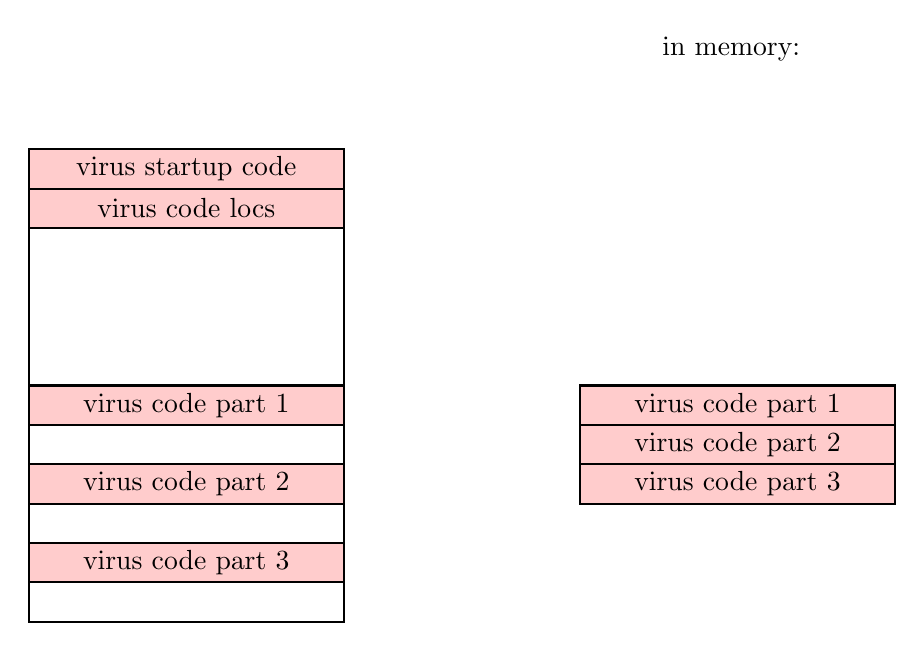
\begin{tikzpicture}
    \draw[fill=red!20,thick] (0, 0) rectangle (4, -0.5) node[midway] {virus startup code};
    \draw[fill=red!20,thick] (0, -0.5) rectangle (4, -1) node[midway] {virus code locs};
    \draw[thick] (0, -1) rectangle (4, -6);
    \draw[fill=red!20,thick] (0, -3) rectangle (4, -3.5)
        node[midway] {virus code part 1};
    \draw[fill=red!20,thick] (0, -4) rectangle (4, -4.5)
        node[midway] {virus code part 2};
    \draw[fill=red!20,thick] (0, -5) rectangle (4, -5.5)
        node[midway] {virus code part 3};
    \begin{scope}[xshift=7cm]
        \node[align=center,anchor=south] at (2, 1) { in memory: };
        \draw[fill=red!20,thick] (0, -3) rectangle (4, -3.5)
            node[midway] {virus code part 1};
        \draw[fill=red!20,thick] (0, -3.5) rectangle (4, -4)
            node[midway] {virus code part 2};
        \draw[fill=red!20,thick] (0, -4) rectangle (4, -4.5)
            node[midway] {virus code part 3};
    \end{scope}
    \end{tikzpicture}
\end{frame}

\begin{frame}{CIH cavities}
    \begin{itemize}
    \item gaps between sections
        \begin{itemize}
        \item common Windows linker aligned sections
        \item (align = start on address multiple of $N$, e.g. $4096$)
        \end{itemize}
    \item reassembling code avoids worrying about splitting instructions
    \end{itemize}
\end{frame}



\subsubsection{segment rounding}
\begin{frame}[fragile]{segment rounding}
\providecommand{\myemphA}[1]{\myemph<2>{#1}}
\providecommand{\myemphB}[1]{\myemph<3>{#1}}
objdump -x /bin/ls: 
\begin{Verbatim}[fontsize=\fontsize{9}{10},commandchars=\\\{\}]
   LOAD off    0x0000000000004000 vaddr 0x0000000000004000 paddr 0x0000000000004000 align 2**12
        filesz \myemphA{0x0000000000013091} memsz 0x0000000000013091 flags r-x
   LOAD off    \myemphB{0x0000000000018000} vaddr 0x0000000000018000 paddr 0x0000000000018000 align 2**12
        filesz 0x0000000000007458 memsz 0x0000000000007458 flags r--
\end{Verbatim}
running /bin/ls in gdb:
\begin{Verbatim}[fontsize=\fontsize{9}{10},commandchars=\\\{\}]
(gdb) info proc map
process 1178818
Mapped address spaces:
          Start Addr           End Addr       Size     Offset  Perms  objfile
      0x555555554000     0x555555558000     0x4000        0x0  r--p   /usr/bin/ls
      0x555555558000     0x55555556c000    \myemphA{0x14000}     0x4000  r-xp   /usr/bin/ls
      0x55555556c000     0x555555574000     0x8000    0x18000  r--p   /usr/bin/ls
....
\end{Verbatim}
\begin{itemize}
\item requested 0x13091 bytes, loaded 0x14000
\item x86-64 Linux: OS allocates only in one page = 4096-byte chunks
\end{itemize}
\end{frame}


\subsection{boot sector}

\againframe<5>{whereCode}

\usetikzlibrary{arrows.meta,chains}

\begin{frame}<1-2>[label=bootProc]{boot process}
    \begin{tikzpicture}
        \begin{scope}[start chain=going below,every node/.style={draw,align=center,join,on chain,thick,minimum width=3.5cm},
                      every join/.style={-Latex,thick}]
        \node[draw=none] (fixedLoc) { processor reset };
        \node[alt=<3>{draw=red,very thick}{}] (bios) {BIOS/EFI \\ \small (chip on motherboard)};
        \node[alt=<2>{draw=red,very thick}{}] (bootloader) {bootloader};
        \node[alt=<4>{draw=red,very thick}{}] (os) {operating system};
        \end{scope}
        \node[left=.5cm of bios,font=\small] (biosLabel) {very CPU/motherboard-specific code};
        \draw[-Latex,thick] (biosLabel) -- (bios);
        \node[left=.5cm of bootloader,font=\small,align=right] (bootloaderLabel) {fixed location on disk \\ code that understands files};
        \draw[-Latex,thick] (bootloaderLabel) -- (bootloader);
        \node[left=.5cm of os,font=\small] (osLabel) {files in a filesystem};
        \draw[-Latex,thick] (osLabel) -- (os);
    \end{tikzpicture}
\end{frame}

\begin{frame}{bootloaders in the DOS era}
    \begin{itemize}
    \item used to be common to boot from floppies
    \item \myemph{default to booting from floppy} if present
        \begin{itemize}
        \item even if hard drive to boot from
        \end{itemize}
    \item applications distributed as bootable floppies
    \item so bootloaders on all devices were a target for viruses
    \end{itemize}
\end{frame}

\begin{frame}{historic bootloader layout}
    \begin{itemize}
    \item bootloader in \myemph{first sector} (512 bytes) of device
    \item (along with partition information)
    \item code in BIOS to copy bootloader into RAM, start running
    \item bootloader responsible for disk I/O etc.
        \begin{itemize}
        \item some library-like functionality in BIOS for I/O
        \end{itemize}
    \end{itemize}
\end{frame}

\begin{frame}{bootloader viruses}
    \newcommand{\tearBox}{
        \draw[very thick] (0, -6) -- (0, 0) -- (4, 0) -- (4, -6);
        \draw[thick] (0, -6) -- (1.2, -5.5) -- (2., -6.6) -- (2.6, -5.8) -- (3.5, -6.6) -- (4, -6);
    }
    \begin{itemize}
    \item example: Stoned
    \end{itemize}
    \begin{tikzpicture}
        \draw[fill=green!20] (0, 0) rectangle (4, -.2);
        \draw[fill=yellow!20] (0, -.2) rectangle (4, -0.5) node[midway,font=\tiny] { partition table };
        \draw[fill=green!20] (0, -.5) rectangle (4, -1.0) node[midway,font=\small] { bootloader };
        \tearBox
        \begin{scope}[xshift=7cm]
        \draw[fill=red!20] (0, 0) rectangle (4, -.2);
        \draw[fill=yellow!20] (0, -.2) rectangle (4, -0.5) node[midway,font=\tiny] { partition table };
        \draw[fill=red!20] (0, -.5) rectangle (4, -1.0) node[midway,font=\small] { virus code };
        \begin{scope}[yshift=-4cm]
        \draw[fill=green!20] (0, 0) rectangle (4, -.2);
        \draw[fill=green!20] (0, -.5) rectangle (4, -1.0) node[midway,font=\small] { saved bootloader };
        \draw[dashed,fill=yellow!20] (0, -.2) rectangle (4, -0.5) node[midway,font=\tiny] { partition table (unused) };
        \end{scope}
        \tearBox 
        \end{scope}
        \draw[line width=1mm,black!50, -Latex] (4.2, -3) -- (6.8, -3);

        \begin{pgfonlayer}{bg}
            \begin{visibleenv}<2>
                \path[fill=blue!30] (0, -4) rectangle (4, -5) node[midway] { data here??? };
            \end{visibleenv}
        \end{pgfonlayer}
    \end{tikzpicture}
\end{frame}

\begin{frame}{data here???}
    \begin{itemize}
        \item might be data there --- risk
        \item some unused space after partition table/boot loader common
            \begin{itemize}
            \item (allegedly)
            \end{itemize}
        \item also be filesystem metadata not used on smaller floppies/disks
        \vspace{.5cm}
        \item but could be wrong --- oops
    \end{itemize}
\end{frame}

\begin{frame}{modern bootloaders --- UEFI}
    \begin{itemize}
    \item BIOS-based boot is going away (slowly)
    \item new thing: UEFI (Universal Extensible Firmware Interface)
    \item like BIOS:
        \begin{itemize}
        \item library functionality for bootloaders
        \item loads initial code from disk/DVD/etc.
        \end{itemize}
    \item unlike BIOS:
        \begin{itemize}
        \item much more understanding of file systems
        \item much more modern set of library calls
        \end{itemize}
    \end{itemize}
\end{frame}

\againframe<3>{bootProc}

\begin{frame}{BIOS/UEFI implants}
    \begin{itemize}
    \item infrequent
    \item BIOS/UEFI code is \myemph{very non-portable}
    \item BIOS/UEFI update may require physical access
    \item BIOS/UEFI code may require cryptographic signatures
    \item \ldots but \myemph{very hard to remove} --- ``persist'' other malware
    \item reports of BIOS/UEFI-infecting ``implants''
        \begin{itemize}
        \item sold by Hacking Team (Milan-based malware company) 
        \item listed in leaked NSA Tailored Access Group catalog
        \end{itemize}
    \end{itemize}
\end{frame}

\againframe<4>{bootProc}

\begin{frame}{system files}
    \begin{itemize}
    \item simpliest strategy: stuff that runs when you start your computer
    \item add a new startup program, run in the background
        \begin{itemize}
        \item easy to blend in
        \end{itemize}
    \vspace{.5cm}
    \item alternatively, infect one of many system programs automatically run
    \end{itemize}

    % FIXME: example from CodeRed or similar?
\end{frame}

 % FIXME: split out UEFI/Secure Boot section

\subsection{memory residence}


\begin{frame}{memory residence}
    \begin{itemize}
    \item malware wants to keep doing stuff
    \item one option --- background process (easy on modern OSs)
    \item also stealthy options:
        \begin{itemize}
        \item insert self into OS code
        \item insert self into other running programs
        \end{itemize}
    \end{itemize}
\end{frame}
 % FIXME: should have more extensive discussion of this somewhere

\section{virus: getting code invoked}


\begin{frame}<1-2>[label=invokeOptions]{invoking virus code: options}
    \begin{itemize}
    \item boot loader
    \item \myemph<2>{change starting location} 
    \item alternative approaches: ``entry point obscuring''
    \item \myemph<3>{edit code that's going to run anyways}
    \item \myemph<4>{replace a function pointer} (or similar)
    \item \ldots
    \end{itemize}
\end{frame}


\subsection{changing start location}


\begin{frame}[fragile,label=invokeStarting]{starting locations}
\begin{Verbatim}[fontsize=\fontsize{10}{11}\selectfont,commandchars=Q\{\}]
/bin/ls:     file format elf64-x86-64
/bin/ls
architecture: i386:x86-64, flags 0x00000112:
EXEC_P, HAS_SYMS, D_PAGED
start address Qmyemph{0x00000000004049a0}
\end{Verbatim}
    \begin{itemize}
    \item modern executable formats have `starting address' field
    \item just change it, insert jump to old address after virus code
    \end{itemize}
\end{frame}




\subsection{overwrite existing code}

\begin{frame}<1>[fragile,label=runAnyways]{run anyways?}
    \begin{itemize}
    \item add code at start of program (Vienna)
        \begin{itemize}
        \item \myemph<2>{plus restore replaced code after running malware code}
        \end{itemize}
    \item return with padding after it:
\begin{Verbatim}[fontsize=\fontsize{10}{11}\selectfont,commandchars=Q\{\}]
  404a01:       c3                      Qtextbf{retq}
  404a02:       0f 1f 40 00             nopl   0x0(%rax)
                Qtextit{replace with}
  404a01:       e9 XX XX XX XX          Qtextbf{jmpq    YYYYYYY}
\end{Verbatim}
        \begin{itemize}
        \item plus return after running malware code
        \end{itemize}
    \item any random place in program?
        \begin{itemize}
        \item just not in the \myemph{middle of instruction}
        \item and \myemph<2>{replace orignal code after running malware code}
        \end{itemize}
    \end{itemize}
\end{frame}

\begin{frame}[fragile,label=findValidChallenge]{challenge: valid locations}
    \begin{itemize}
    \item x86: probably don't want a full instruction parser
    \item x86: might be non-instruction stuff mixed in with code:
\begin{lstlisting}[language=myasm,style=smaller]
do_some_floating_point_stuff:
            movss float_one(%rip), %xmm0
            ...
            retq
float_one: .float 1
\end{lstlisting}
    \begin{itemize}
        \item floating point value one ({\tt 00 00 80 3f}) is not valid machine code
        \item disassembler might lose track of instruction boundaries
    \end{itemize}
    \end{itemize}
\end{frame}

\begin{frame}[fragile,label=findValidFindFunc]{finding function calls}
    \begin{itemize}
    \item one idea: replace calls
    \item normal x86 call FOO: {\tt E8 \textit{(32-bit value: PC - address of foo)}}
    \item could look for E8 in code --- \myemph{lots of false positives}
        \begin{itemize}
        \item probably even if one excludes out-of-range addresses
        \end{itemize}
    \end{itemize}
\end{frame}

\begin{frame}[fragile,label=findValidFindFunc2]{really finding function calls (1)}
\lstset{language=myasm,style=small}
    \begin{itemize}
    \item e.g. some popular compilers started x86-32 functions with
\begin{lstlisting}
foo:
    push %ebp       // push old frame pointer
    // 0x55
    mov %esp, %ebp  // set frame pointer to stack pointer
    // 0x89 0xec
\end{lstlisting}
    \item use to identify when {\tt e8} refers to real function
    \begin{itemize}
    \item (full version: also have some other function start patterns)
    \end{itemize}
    \end{itemize}
\end{frame}

\begin{frame}{really finding function calls (2)}
    \begin{itemize}
    \item x86-64 assembly seen a lot of ENDBR64 (hex {\tt f3 0f 1e fa})
    \item marker for valid locations to jump to
        \begin{itemize}
        \item intention: part of possible defense against return-oriented-programming-style attacks
        \item (we'll talk about what this means later)
        \end{itemize}
    \item likely only seen at beginning of functions, switch statement cases, etc.
    \end{itemize}
\end{frame}

\againframe<2>{runAnyways}

\begin{frame}{restoring replaced code?}
    \begin{itemize}
    \item Vienna: just write to memory addres
    \vspace{.5cm}
    \item modern OS: segfault/general protection fault
        \begin{itemize}
        \item code loaded read-only
        \end{itemize}
    \item easy solution: make library call to make it writable
        \begin{itemize}
        \item Linux: \texttt{mprotect}
        \item functionality exists to, e.g., allow compiling code at runtime
        \end{itemize}
    \end{itemize}
\end{frame}


\subsection{using dynamic linking features}

\begin{frame}{infecting shared libraries via relocations}
\begin{tikzpicture}
    \draw[thick] (0, 0) rectangle (4, -6) coordinate (bottomRight) node[midway] { \tt kernel32.dll };
    \draw[thick,fill=yellow!20] (0, 0) rectangle (4, -0.5) node[midway,font=\small] {header};
    \draw[thick,fill=blue!20] (0, -0.5) rectangle (4, -2.0);
    \node[font=\small,anchor=north] at (2, -0.5) {symbol table};
    \node[anchor=north west,font=\fontsize{9}{10}\selectfont] (GFAName) at (0, -0.9) {
        \tt GetFileAttributesA
    };
    \node[anchor=north west] at (GFAName.south west) {\tt \ldots};
    \draw[-Latex,thick] ([xshift=.5mm]GFAName.east) coordinate (startArrowA) -- ([xshift=.5cm]GFAName.west -| bottomRight) |- (3, -5);
    \fill[black] (startArrowA) circle[radius=.5mm];

    \draw[line width=2mm,-Latex,black!60] (4.6, -3) -- (6.9, -3);
    \begin{scope}[xshift=7cm]
    \draw[thick] (0, 0) rectangle (4, -6) coordinate (bottomRight) node[midway] { \tt kernel32.dll };
    \draw[thick,fill=yellow!20] (0, 0) rectangle (4, -0.5) node[midway,font=\small] {header};
    \draw[thick,fill=blue!20] (0, -0.5) rectangle (4, -2.0);
    \node[font=\small,anchor=north] at (2, -0.5) {symbol table};
    \draw[thick,fill=red!20] (0, -6) rectangle (4, -7) node[midway,font=\small] {virus code};
    \node[anchor=north west,font=\fontsize{9}{10}\selectfont] (GFANameB) at (0, -0.9) {
        \tt GetFileAttributesA
    };
    \node[anchor=north west] at (GFANameB.south west) {\tt \ldots};
    \draw[-Latex,very thick,red] ([xshift=.5mm]GFANameB.east) coordinate (startArrowA) -- ([xshift=.5cm]GFANameB.west -| bottomRight) |- (1, -6.2);
    \fill[red] (startArrowA) circle[radius=.5mm];
    \end{scope}
\end{tikzpicture}
\end{frame}

\begin{frame}{other dynamic-linking-based infections}
    \begin{itemize}
    \item could also modify
    \vspace{.5cm}
    \item relocations on executable
        \begin{itemize}
        \item this isn't the table entry for \texttt{puts}, \\ it's the one for \texttt{evilvirus}
        \end{itemize}
    \item list of needed libraries?
        \begin{itemize}
        \item the C standard library and virus.so
        \end{itemize}
    \item stubs and calls to stub
        \begin{itemize}
        \item very regular and easy to locate
        \end{itemize}
    \end{itemize}
\end{frame}
 % FIXME: 20.04 example?

% FIXME: discussion about hiding worm-like programs?

\section{virus summary?}


\begin{frame}{summary}
    \begin{itemize}
    \item how to hide:
        \begin{itemize}
        \item separate executable
        \item append
        \item existing ``unused'' space
        \item append + compression
        \end{itemize}
    \item how to run:
        \begin{itemize}
        \item change entry point (start address)
        \item change calls
        \item change beginning of function
        \item change dynamic-linking-related pointers
        \item arrange to run as part of OS
        \end{itemize}
    \end{itemize}
\end{frame}


\begin{frame}{upcoming assignment}
    \begin{itemize}
    \item TRICKY
    \item insert `virus' code at specific point in 3 related executables
        \begin{itemize}
        \item should make executable print message from `virus' code at specific point
        \end{itemize}
    \item recommended method: replacing function returns
    \end{itemize}
\end{frame}

\section{discussion question}
\begin{frame}{virus: easiest code to find?}
    \begin{itemize}
    \item what should be easiest/hardest to identify \\
        without many false positives?
        \item A. replaced start location
        \item B. replaced dynamic linker stub
        \item C. replaced dynamic library symbol location
        \item D. replaced function call
        \item E. replaced function return
        \item F. replaced bootloader
        \item G. new automatically started system program
    \end{itemize}
\end{frame}




\section{why don't viruses\ldots}
\usetikzlibrary{shapes.callouts}

\begin{frame}<1>[fragile,label=whyChoices]{virus choices?}
\begin{itemize}
\item why don't viruses always append/replace\tikzmark{append}?
\item why don't viruses always change start location\tikzmark{start}?
\item why did I bother talking about all these strategies?
\end{itemize}
\begin{tikzpicture}[overlay,remember picture]
\coordinate (calloutLoc) at ([yshift=-2cm]current page.center);
\begin{visibleenv}<2>
    \node[my callout=append] at (calloutLoc) {
        head/tail scanning? 
    };
\end{visibleenv}
\begin{visibleenv}<3>
    \node[my callout=start]  at (calloutLoc){
        check for suspicious starting location?
    };
\end{visibleenv}
\end{tikzpicture}
\end{frame}

\begin{frame}{more on virus strategies}
    \begin{itemize}
    \item after we talk about anti-virus strategies some
    \end{itemize}
\end{frame}



\section{the cat and mouse game}
\usetikzlibrary{shapes.misc}

{ % all template changes are local to this group.
    \setbeamertemplate{navigation symbols}{}
    \contourlength{.2mm}
    \begin{frame}[plain]
        \begin{tikzpicture}[remember picture,overlay]
            \node[at=(current page.center)] (image) {
                
\includegraphics[height=\paperheight]{../heur-detect/1600x1200-Tom-Jerry-Chase}
            };
            %\draw[help lines] (0, 0) grid (12, -8);
            \begin{scope}[shift={([yshift=-0.75cm,xshift=1cm]image.north west)}]
            \node[cross out,draw,line width=1mm,black,at={(9,-6)},anchor=center,minimum width=6cm,minimum height=1.25cm] {};
            \node[at={(3,-8.25)},anchor=center,font=\Huge\bfseries,
                red!90!black,align=left] {\contour{black}{Anti-\hspace{-.4ex}Virus}};
            \node[at={(6.5,-8.25)},anchor=center,font=\large\bfseries,
                red!90!black,align=left,rotate=30] {\contour{black}{and}};
            \node[at={(8.5,-8.25)},anchor=center,font=\Huge\bfseries,
                red!90!black,align=left] {\contour{black}{Virus}};
            \end{scope}
        \end{tikzpicture}
     \end{frame}
}




\section{antimalware goals}

\begin{frame}{anti-malware software goals}
    \begin{itemize}
    \item prevent malware from running
    \item prevent malware from spreading
    \item undo the effects of malware
    \vspace{.5cm}
    \item<2-> key subproblem: detect malware
    \end{itemize}
\end{frame}



\section{simple detection: tripwire} 
    % FIXME: tripwire
\begin{frame}{tripwire}
    \begin{itemize}
    \item open source tool from c. 2000
        \begin{itemize}
        \item also company around that tool, but I don't know about it
        \end{itemize}
    \item ``tool for monitoring and alerting on file \& directory changes''
    \item targetted at servers with professional administrators
    \vspace{.5cm}
    \item setup: run tool, it records state of system/etc. files (e.g. hashes)
    \item later: run tool, it tells you if anything changed
    \end{itemize}
\end{frame}

\begin{frame}{tripwire as antimalware software?}
    \begin{itemize}
    \item tripwire idea: detect any changes
    \item notify user (administrator) about them
    \vspace{.5cm}
    \item what is user supposed to do with this info?
    \vspace{.5cm}
    \item what about normal software updates, etc.?
    \item can malware hide in files that are supposed to change?
        \begin{itemize}
        \item ``data'' files with other programs, scripts?
        \item \ldots
        \end{itemize}
    \item what if system compromised before setup?
    \end{itemize}
\end{frame}


\section{application whitelisting: AppLocker}
\begin{frame}{application whitelisting}
\begin{itemize}
\item how about we only let standard applications run, unmodified?
    \begin{itemize}
    \item AppStore-based strategy?
    \end{itemize}
\item not uncommon in corporate environments:
\end{itemize}
\vspace{.5cm}
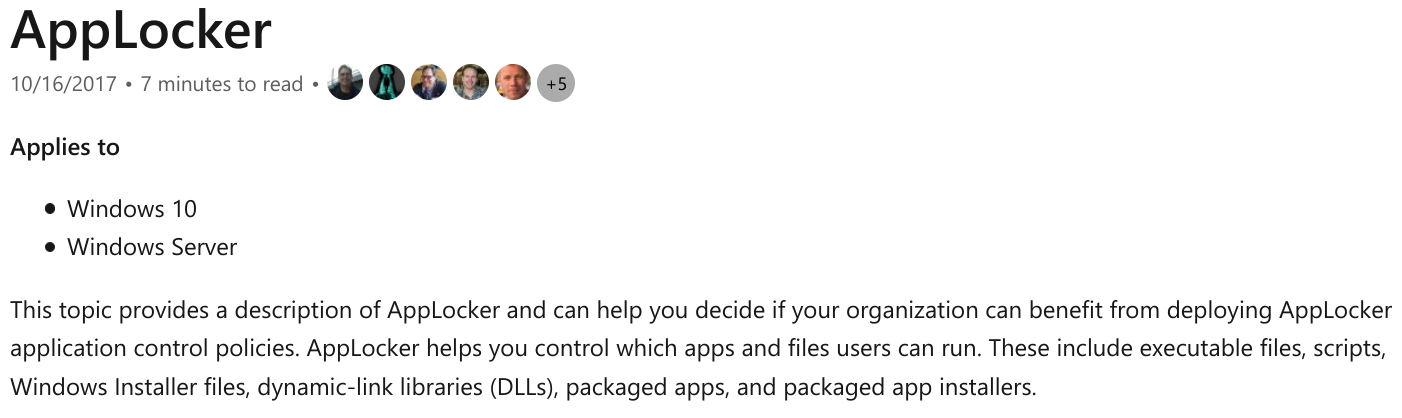
\includegraphics[width=\textwidth]{../heur-detect/applocker-manual}
\end{frame}

\begin{frame}{case study: Microsoft AppLocker}
    \begin{itemize}
    \item AppLocker is Windows 7+ feature for limiting what can run
        \begin{itemize}
        \item successor(?) feature App Control for Business (Windows 10+)
        \end{itemize}
    \item adminstrator sets rules about\ldots
    \item what publisher is allowed
        \begin{itemize}
        \item publisher cryptographically signs applications
        \item virus-like techniques break signatures
        \item allows upgrades!
        \end{itemize}
    \item what file hashes are allowed
        \begin{itemize}
        \item requires manual update each time software updates
        \end{itemize}
    \item what locations are allowed
        \begin{itemize}
        \item presumably for administrator-only directories
        \end{itemize}
    \end{itemize}
\end{frame}

\begin{frame}{problems with whitelisting}
    \begin{itemize}
    \item programs with features/bugs malware could exploit
        \begin{itemize}
        \item ``AppLocker does not control the behavior of applications after they are launched. Applications could contain flags passed to functions that signal AppLocker to circumvent the rules and allow another .exe or .dll to be loaded.''
        \end{itemize}
    \item users want to install/develop other software
    \item scripting:
        \begin{itemize}
        \item ``Not all host processes call into AppLocker and, therefore, AppLocker cannot control every kind of interpreted code''
        \end{itemize}
    \end{itemize}
\end{frame}


\section{secure boot}

\begin{frame}{modern bootloaders --- secure boot}
    \begin{itemize}
    \item ``Secure Boot'' is a common feature of modern bootloaders
    \item idea: UEFI/BIOS code checks bootloader code, fails if not okay
        \begin{itemize}
        \item requires user intervention to use not-okay code
        \end{itemize}
    \end{itemize}
\end{frame}

\begin{frame}{Secure Boot and keys}
    \begin{itemize}
    \item Secure Boot relies on cryptographic signatures
        \begin{itemize}
        \item idea: accept only ``legitimate'' bootloaders
        \item legitimate: known authority vouched for them
        \end{itemize}
    \item user control of their own systems?
        \begin{itemize}
        \item in theory: can add own keys
        \end{itemize}
    \item what about changing OS instead of bootloader?
        \begin{itemize}
        \item bootloader could check cryptographic signature or hash of kernel being loaded
        \end{itemize}
    \end{itemize}
\end{frame}




\section{signature-based detection, generally}
% FIXME: key idea: in files


\begin{frame}{malware ``signatures''}
    \begin{itemize}
    \item typically can't rely on whitelisting approach
        \begin{itemize}
        \item software and related files change legitimately
        \item (note: malware might not be in main executables)
        \end{itemize}
    \vspace{.5cm}
    \item antivirus vendor have \myemph{signatures} for known malware
    \item many options to represent signatures
    \item thought process: \myemph{signature for Vienna?}
    \vspace{.5cm}
    \item goals: compact, fast to check, reliable
    \end{itemize}
\end{frame}



\subsection{detecting Vienna exercise?}
\begin{frame}{what signature for Vienna?}
    \begin{itemize}
    \item Suppose we wanted to detect Vienna in execs.
    \item What is best to look for in an exectuable\ldots \\
        in terms of performance? false positives? true positives?
        \begin{itemize}
        \item A. machine code found in example infected file at the end of the executable 
        \item B. machine code found in example infected file at the end of the executable, ignoring parts that change on reinfection
        \item C. portion of virus's machine code that copies itself to a new file anywhere in the executable
        \item D. whether another executable file in same directory changes if we run the executable in a VM
        \item E. for a jump at beginning of the executable to something near the end
        \end{itemize}
    \end{itemize}
\end{frame}


\subsection{case study: Vienna}

\begin{frame}[fragile,label=viennaSigs]{exercise: signatures for Vienna}
\lstset{
        style=smaller,
        language=myasm,
        moredelim={**[is][\btHL<2|handout:0>]{~2~}{~end~}},
        moredelim={**[is][\btHL<3|handout:0>]{~3~}{~end~}},
        moredelim={**[is][\btHL<3-4|handout:0>]{~34~}{~end~}},
        moredelim={**[is][\btHL<4|handout:0>]{~4~}{~end~}},
        }
\begin{tabular}{l@{\hspace{1cm}}ll}
\begin{lstlisting}
~2~jmp 0x0700~end~ /* C */
mov $0x9e4e, %si /* A */
...              /* A */
/* more app code */ 
...              /* A */
~3~push %cx~end~
mov $0x8f9, %si /* C */
...
mov $0x0100, %di
mov $3, %cx
rep movsb
...
\end{lstlisting}
&
\begin{lstlisting}
...
add $0x2f9, %cx
mov %si, %di
sub $0x1f7, %di
mov %cx, (%di)
...
mov $0x288, %cx
mov $0x40 %ah
mov $si, $dx
sub $0x1f9, %dx
int 0x21
...
\end{lstlisting}
&
\begin{lstlisting}
pop %cx
xor %ax, %ax
xor %bx, %bx
~4~xor %dx, %dx~end~
~4~mov $0x0100, %di~end~
~4~push %di~end~
~4~xor %di, %di~end~
~34~ret~end~
/* virus data */
\end{lstlisting}
\\
\end{tabular}
\verb|/* C */| = constant changes when Vienna relocated \\
\verb|/* A */| = application code
\end{frame}

\begin{frame}{simple signature (1)}
    \begin{itemize}
    \item all the code Vienna copies
    \item \ldots{} except changed {\tt mov} to {\tt \%si}
    \vspace{.5cm}
    \item virus doesn't change it to relocate
    \item includes infection code --- definitely malicious
    \end{itemize}
\end{frame}

\begin{frame}{signature generality}
    \begin{itemize}
    \item the Vienna virus was copied a bunch of times
    \item small changes, ``payloads'' added
        \begin{itemize}
        \item print messages, do different malicious things, \ldots
        \end{itemize}
    \item this signature will not detect any variants
    \item can we do better?
    \end{itemize}
\end{frame}

\begin{frame}{simple signature (2)}
    \begin{itemize}
    \item Vienna start code
        \begin{itemize}
        \item weird jump at beginning??
        \end{itemize}
    \item problem: maybe real applications do this?
    \item problem: easy to move jump
    \end{itemize}
\end{frame}

\begin{frame}{simple signature (3)}
    \begin{itemize}
    \item Vienna infection code
        \begin{itemize}
        \item scans directory, finds files
        \end{itemize}
    \item likely to stay the same in variants?
    \item<2> problem: virus writers \myemph{react to antivirus}
    \end{itemize}
\end{frame}

\begin{frame}{simple signature (4)}
    \begin{itemize}
    \item Vienna finish code
        \begin{itemize}
        \item push + ret 
        \end{itemize}
    \item very unusual pattern
    \item probably(?) not in ``real'' programs
    \item real effort to change to something else?
    \item<2> problem: virus writers \myemph{react to antivirus}
    \end{itemize}
\end{frame}




\subsection{difficult goals for signatures}

\begin{frame}{making things hard for the mouse}
    \begin{itemize}
    \item don't want \myemph{trivial changes} to break detection
    \item want to detect \myemph{strategies}
        \begin{itemize}
        \item e.g. require changing relocation logic
        \item \ldots not just reordering instructions, adding nops
        \end{itemize}
    \item need to detect signatures in real time
        \begin{itemize}
        \item don't want interrupt user (much)
        \end{itemize}
    \item want to avoid false positive
    \item goals: compact, fast to check, reliable, \myemph{general?}
    \end{itemize}
\end{frame}



\subsection{Vienna: general pattern?}
     % FIXME: more examples of general things Vienna does

\begin{frame}{generic pattern example}
    \begin{itemize}
    \item another possibility: detect writing near {\tt 0x100}
    \item {\tt 0x100} was DOS program entry code  --- no program should do this(?)
    \item problem: how to represent this?
    \begin{itemize}
        \item describe machine code bytes
        \item multiple possibilities
        \end{itemize}
    \end{itemize}
\end{frame}


\section{regular expressions}

\begin{frame}{regular expressions}
    \begin{itemize}
    \item one method of representing patterns like this: \\
          regular expressions (regexes)
    \item restricted language allows very fast implementations
        \begin{itemize}
        \item especially when there's a long list of patterns to look for
        \end{itemize}
    \item homework assignment next week
    \end{itemize}
\end{frame}

\begin{frame}{regular expressions: implementations}
    \begin{itemize}
    \item multiple implementations of regular expressions
    \item we will target: flex, a parser generator
    \end{itemize}
\end{frame}

\begin{frame}[fragile,label=simplePat]{simple patterns}
    \begin{itemize}
    \item alphanumeric characters \myemph{match themselves}
    \item {\tt foo}:
        \begin{itemize}
        \item matches exactly {\tt foo} only
        \item does not match {\tt Foo}
        \item does not match \verb*|foo |
        \item does not match {\tt foobar}
        \end{itemize}
    \item backslash might be needed for others
    \item \verb|C\+\+|
        \begin{itemize}
        \item matches exactly {\tt C++} only
        \end{itemize}
    \end{itemize}
\end{frame}

\begin{frame}[fragile,label=meta1]{metachars (1)}
    \begin{itemize}
    \item special ways to match characters
    \vspace{.5cm}
    \item \verb|\n|, \verb|\t|, \verb|\x3C|, \ldots --- work like in C
    \item \verb|[b-fi]| --- {\tt b} or {\tt c} or {\tt d} or {\tt e} or {\tt f} or {\tt i}
    \item \verb|[^b-fi]| --- any character but {\tt b} or {\tt c} or \ldots
    \item {\tt .} --- any character except newline
    \item \verb!(.|\n)! --- any character
    \end{itemize}
\end{frame}

\begin{frame}[fragile,label=meta2]{metachars (2)}
    \begin{itemize}
    \item \verb|a*| --- zero or more as:
        \begin{itemize}
        \item (empty string), {\tt a}, {\tt aa}, {\tt aaa}, \ldots
        \end{itemize}
    \item \verb|a{3,5}| --- three to five as:
        \begin{itemize}
        \item {\tt aaa}, {\tt aaaa}, {\tt aaaaa}
        \end{itemize}
    \item \verb!(abc){3,5}! --- three to five abcs: (``grouping'')
        \begin{itemize}
        \item {\tt abcabcabc}, {\tt abcabcabcabc}, {\tt abcabcabcabcabc}
        \end{itemize}
    \item {\tt ab|cd}
        \begin{itemize}
        \item {\tt ab}, {\tt cd}
        \end{itemize}
    \item \verb!(ab|cd){2}! --- two ab-or-cds:
        \begin{itemize} 
        \item {\tt abab}, {\tt abcd}, {\tt cdab}, {\tt cdcd}
        \end{itemize}
    \end{itemize}
\end{frame}

\begin{frame}[fragile,label=meta3]{metachars (3)}
    \begin{itemize}
    \item \verb|\xAB| --- the byte {\tt 0xAB}
    \item \verb|\x00| --- the byte {\tt 0x00}
        \begin{itemize}
        \item flex is designed for text, handles binary fine
        \end{itemize}
    \item \verb|\n| --- newline (and other C string escapes)
    \end{itemize}
\end{frame}

\begin{frame}[fragile,label=example1]{example regular expressions}
    \begin{itemize}
    \item match words ending with {\tt ing}: \\
        \verb|[a-zA-Z]*ing|
    \item match C {\tt /* ... */} comments: \\
        \verb!/\*([^*]|\*[^/])*\*/!
    \end{itemize}
\end{frame}




\subsection{flex example}
\usetikzlibrary{fit}

\begin{frame}{flex}
    \begin{itemize}
    \item flex is a regular expression matching tool
    \item intended for writing \myemph{parsers}
    \item generates \myemph{C code}
    \item parser function called {\tt yylex}
    \end{itemize}
\end{frame}


\begin{frame}[fragile,label=flexEx]{flex example}
\lstset{style=small,language={}}
\begin{tikzpicture}
\begin{scope}
\tikzset{every node/.style={font=\small,align=left,anchor=north west,inner sep=0mm}}
\node (vars) {
\begin{lstlisting}
        int num_bytes = 0, num_lines = 0;
        int num_foos = 0;
\end{lstlisting}
};
\node (patMacros) at (vars.south west) {
~
};
\node (sepA) at (patMacros.south west) {
\begin{lstlisting}
%%
\end{lstlisting}
};
\node (pats) at (sepA.south west) {
\begin{lstlisting}
foo     { 
          num_bytes += 3;
          num_foos += 1;
        }
.       { num_bytes += 1; }
\n      { num_lines += 1; num_bytes += 1; }
\end{lstlisting}
};
\node (sepB) at (pats.south west) {
\begin{lstlisting}
%%
\end{lstlisting}
};
\node (mainCode) at (sepB.south west) {
\begin{lstlisting}
int main(void) {
    yylex();
    printf("%d bytes, %d lines, %d foos\n",
           num_bytes, num_lines, num_foos);
}
\end{lstlisting}
};
\end{scope}

\tikzset{
    hi/.style={rounded corners,fill=green,opacity=0.3},
    remark/.style={draw,red,very thick,at={([xshift=-3cm]pats.east)},fill=white,align=left},
    remark2/.style={draw,red,very thick,at={([xshift=-3cm,yshift=2cm]pats.east)},fill=white,align=left},
}

\begin{visibleenv}<2>
    \node[hi,fit=(sepA)] {};
    \node[hi,fit=(sepB)] {};
    \node[remark] {three sections};
\end{visibleenv}

\begin{visibleenv}<3>
    \node[hi,fit=(vars)] {};
    \node[remark] {first --- declarations for later \\
                   C code in output file};
\end{visibleenv}

\begin{visibleenv}<4>
    \node[hi,fit=(pats)] {};
    \node[remark2] {patterns, code to run on match \\
                   as parser: return ``token'' here};
\end{visibleenv}

\begin{visibleenv}<5>
    \node[hi,fit=(mainCode)] {};
    \node[remark] {extra code to include};
\end{visibleenv}

\end{tikzpicture}
\end{frame}

\begin{frame}[fragile,label=flexMatched]{flex: matched text}
\lstset{
        style=small,
        language={},
        moredelim={**[is][\btHL<2|handout:0>]{~2~}{~end~}},
        }
\begin{tikzpicture}
\begin{scope}
\tikzset{every node/.style={font=\small,align=left,anchor=north west,inner sep=0mm}}
\node (vars) {
\begin{lstlisting}
\end{lstlisting}
};
\node (patMacros) at (vars.south west) {
~
};
\node (sepA) at (patMacros.south west) {
\begin{lstlisting}
%%
\end{lstlisting}
};
\node (pats) at (sepA.south west) {
\begin{lstlisting}
[aA][a-z]* {
               printf("found a-word '%s'\n",
                      ~2~yytext~end~);
           }
(.|\n)     {} /* default rule: would output text */
\end{lstlisting}
};
\node (sepB) at (pats.south west) {
\begin{lstlisting}
%%
\end{lstlisting}
};
\node (mainCode) at (sepB.south west) {
\begin{lstlisting}
int main(void) {
    yylex();
}
\end{lstlisting}
};
\end{scope}
\tikzset{
    hi/.style={rounded corners,fill=green,opacity=0.3},
    remark/.style={draw,red,very thick,at={([xshift=-4cm,yshift=2cm]pats.east)},fill=white,align=left},
}
\begin{visibleenv}<2>
    \node[remark] {yytext --- text of matched thing};
\end{visibleenv}
\end{tikzpicture}
\end{frame}


\begin{frame}[fragile,label=flexDef]{flex: definitions}
\lstset{
        style=small,
        language={},
        moredelim={**[is][\btHL<2|handout:0>]{@hi2@}{@endhi@}},
        }
\begin{tikzpicture}
\begin{scope}
\tikzset{every node/.style={font=\small,align=left,anchor=north west,inner sep=0mm}}
\node (vars) {
\begin{lstlisting}
\end{lstlisting}
};
\node (patMacros) at (vars.south west) {
\begin{lstlisting}
A        [aA]
LOWERS   [a-z]
ANY      (.|\n)
\end{lstlisting}
};
\node (sepA) at (patMacros.south west) {
\begin{lstlisting}
%%
\end{lstlisting}
};
\node (pats) at (sepA.south west) {
\begin{lstlisting}
{A}{LOWERS}* {
                printf("found a-word '%s'\n",
                       yytext);
             }
{ANY}        {} /* default rule would
                   output text */
\end{lstlisting}
};
\node (sepB) at (pats.south west) {
\begin{lstlisting}
%%
\end{lstlisting}
};
\node (mainCode) at (sepB.south west) {
\begin{lstlisting}
int main(void) {
    yylex();
}
\end{lstlisting}
};
\end{scope}
\tikzset{
    hi/.style={rounded corners,fill=green,opacity=0.3},
    remark/.style={draw,red,very thick,at={([xshift=-4cm,yshift=2cm]pats.east)},fill=white,align=left},
}
\begin{visibleenv}<2>
    \node[hi,fit=(patMacros)] {};
    \node[remark] {definitions of common patterns \\ included later};
\end{visibleenv}
\end{tikzpicture}
\end{frame}


\subsection{flex state machines}

\usetikzlibrary{arrows,automata}

\begin{frame}[fragile,label=flexSM]{flex: state machines}
\lstset{
        style=small,
        language={},
        moredelim={**[is][\btHL<2|handout:0>]{@hi2@}{@endhi@}},
        }
\begin{tikzpicture}
\node (flexStuff) {
\begin{lstlisting}
foo     {...}
.       {...}
\n      {...}
\end{lstlisting}
};
\begin{scope}[every node/.style={font=\tt,thick}]
\node[initial, state,below=1cm of flexStuff,font=\normalfont\it] (start) {};
\node[state,right=1cm of start] (f) {f};
\node[state,right=1cm of f] (fo) {fo};
\node[state,right=1cm of fo,accepting] (foo) {foo};
\node[state,below right=2cm of start,accepting] (dot) {.};
\node[state,below=1.5cm of start,accepting] (newline) {\textbackslash{}n};
\end{scope}
\path[-Latex,thick] (start) edge node[above] {\tt f} (f)
                    (f) edge node[above] {\tt o} (fo)
                    (fo) edge node[above] {\tt o} (foo)
                    (start) edge node[sloped,above] {other} (dot)
                    (start) edge node[left] {\textbackslash{}n} (newline);
\begin{visibleenv}<2>
    \path[-Latex,blue,dashed] (f) edge node[right] {(back 1)} (dot);
    \path[-Latex,blue,dashed] (fo) edge[out=-45,in=-30] node[midway, sloped, below] {(back 2)} (dot);
\end{visibleenv}
\end{tikzpicture}
\end{frame}

\begin{frame}[fragile,label=stateMachineMatch]{state machine matching}
\begin{tikzpicture}
\node(matchString) {\large \tt \sout<3->{\myemph<2>{a}}\sout<4->{b}\sout<7->{\myemph<5-6>{f}\myemph<6>{oo}}\myemph<7-8>{f}\myemph<7>{\sout<8>{o}}abffoo};

\begin{scope}[every node/.style={font=\tt,thick}]
\node[initial, state,below=1cm of matchString,font=\normalfont\it,
      alt=<2>{red}{}] (start) {};
\node[state,right=1cm of start,alt={<5,7>{red}{}}] (f) {f};
\node[state,right=1cm of f,alt={<6,7>{red}{}}] (fo) {fo};
\node[state,right=1cm of fo,accepting,alt={<6>{red}{}}] (foo) {foo};
\node[state,below right=2cm of start,accepting,alt={<3,8>{red}{}}] (dot) {.};
\node[state,below=1.5cm of start,accepting] (newline) {\textbackslash{}n};
\end{scope}
\path[-Latex,thick] (start) edge[alt=<5-7>{red}{}] node[above] {\tt f} (f)
                    (f) edge node[above,alt=<6>{red}{}] {\tt o} (fo)
                    (fo) edge node[above,alt=<6>{red}{}] {\tt o} (foo)
                    (start) edge node[sloped,above,alt=<3>{red}{}] {other} (dot)
                    (start) edge node[left] {\textbackslash{}n} (newline);
\path[-Latex,blue,dashed] (f) edge node[right] {(back 1)} (dot);
\path[-Latex,blue,dashed,alt=<8>{red,thick}{}] (fo) edge[out=-45,in=-30] node[midway, sloped, below] {(back 2)} (dot);
\end{tikzpicture}
\end{frame}





\begin{frame}{why this?}
    \begin{itemize}
    \item one pass matching (except for some backtracking)
        \begin{itemize}
        \item can make state machine bigger to avoid some backtracking
        \end{itemize}
    \item basically speed of file I/O
    \item handles multiple patterns well
    \item flexible for ``special cases''
    \vspace{.5cm}
    \item<2> real anti-virus: probably custom pattern ``engine''
    \end{itemize}
\end{frame}




\subsection{backtracking problems?}

\usetikzlibrary{arrows.meta,automata,positioning}
\begin{frame}[fragile,label=flexHow]{precomputing backtracking}
\lstset{
        style=small,
        language={},
        moredelim={**[is][\btHL<2|handout:0>]{@hi2@}{@endhi@}},
        }
\begin{tikzpicture}
\node (flexStuff) {
\begin{lstlisting}
foo     {...}
.       {...}
\n      {...}
\end{lstlisting}
};
\begin{scope}[every node/.style={font=\tt,thick}]
\node[initial, state,below=1cm of flexStuff,font=\normalfont\it] (start) {};
\node[state,right=1cm of start] (f) {f};
\node[state,right=1cm of f] (fo) {fo};
\node[state,right=1cm of fo,accepting] (foo) {foo};
\node[state,below right=2cm of start,accepting] (dot) {.};
\node[state,below=1.5cm of start,accepting] (newline) {\textbackslash{}n};
\end{scope}
\path[-Latex,thick] (start) edge node[above] {\tt f} (f)
                    (f) edge node[above] {\tt o} (fo)
                    (fo) edge node[above] {\tt o} (foo)
                    (start) edge node[sloped,above] {other} (dot)
                    (start) edge node[right] {\textbackslash{}n} (newline);
\path[-Latex,red,draw,very thick,dashed] (f) -- node[midway,above,sloped]{other} ++ (3cm, -2cm) node[below,draw,align=left] {match \texttt{.} once \\ for \texttt{f}, \\ goto start};
\path[-Latex,red,draw,very thick,dashed] (fo) -- node[midway,above,sloped]{other} ++ (4cm, -2cm) node[below,draw,align=left] {match \texttt{.} twice \\ for \texttt{fo}, \\ goto start};
\end{tikzpicture}
\end{frame}




\usetikzlibrary{arrows.meta,automata,positioning}

\begin{frame}[fragile,label=noBt]{avoiding backtracing?}
\lstset{
        style=small,
        language={},
        moredelim={**[is][\btHL<2|handout:0>]{@hi2@}{@endhi@}},
        }
\begin{tikzpicture}
\node (flexStuff) {
\begin{lstlisting}
fox  {...}
foo  {...}
off  {...}
.|\n {/* do nothing */}
\end{lstlisting}
};
\begin{scope}[every node/.style={font=\tt,thick}]
\node[initial, state,below=2cm of flexStuff,font=\normalfont\it] (start) {};
\node[state,above right=1cm of start] (f) {f};
\node[state,right=1cm of f] (fo) {fo};
\node[state,above right=1cm of fo,accepting] (fox) {fox};
\node[state,right=1cm of fo,accepting] (foo) {foo};
\node[state,below right=1cm of start] (o) {o};
\node[state,right=1cm of o] (of) {of};
\node[state,right=1cm of of,accepting] (off) {off};
\end{scope}
\path[-Latex,thick]
                    (start) edge[loop below] node[below] {other} (start);
\path[-Latex,thick]
                    (start) edge node[above] {\tt f} (f)
                    (f) edge node[above] {\tt o} (fo)
                    (fo) edge node[above] {\tt o} (foo)
                    (fo) edge node[above] {\tt x} (fox)
                    (start) edge node[above] {\tt o} (o)
                    (o) edge node[above] {\tt f} (of)
                    (of) edge node[above] {\tt f} (off);
\path[red,-Latex,thick] (f) edge node[right,align=left] {\tt o} (o);
\path[red,-Latex,thick] (of) edge node[right,align=left] {\tt o} (f);
\path[red,-Latex,thick] (fo) edge node[right,align=left] {\tt f} (of);
\end{tikzpicture}
\end{frame}



\subsection{flex: Vienna example}

\begin{frame}[fragile,label=ViennaPat1]{Vienna patterns (1)}
\lstset{
        style=small,
        language={},
        moredelim={**[is][\btHL<2|handout:0>]{@hi2@}{@endhi@}},
        escapechar=`,
        }
\begin{itemize}
\item simple Vienna patterns:
\end{itemize}
\begin{lstlisting}
/* bytes of fixed part of Vienna sample */
\xFC\x89\xD6\x83\xC6\x81\xc7\x00\x01\x83`\textit{(etc)}` {
        printf("found Vienna code\n");
    }
\end{lstlisting}
\end{frame}


\begin{frame}[fragile,label=ViennaPat2]{Vienna patterns (2)}
\lstset{
        style=small,
        language={},
        moredelim={**[is][\btHL<2|handout:0>]{@hi2@}{@endhi@}},
        escapechar=`,
        }
\begin{itemize}
\item simple Vienna patterns:
\end{itemize}
\begin{lstlisting}
/* Vienna sample with wildcards for
   changing bytes: */
/* push %CX; mov ???, %dx; cld; ... */
\x51\xBA@hi2@(.|\n)(.|\n)@endhi@\xFC\x89`\textit{(etc)}` {
        printf("found Vienna code w/placeholder\n");
    }
/* mov $0x100, %di; push %di; xor %di, %di; ret */
\xBF\x00\x01\x57\x31\xFF\xC3 {
        printf("found Vienna return code\n");
    }
\end{lstlisting}
\end{frame}




\subsection{why the flexibility?}
\begin{frame}{regular expressions are flexible}
    \begin{itemize}
    \item for Vienna: lots of flex features we didn't need
        \begin{itemize}
        \item things being repeated variable number of times
        \item one of list of possible characters (bytes)
        \item \ldots
        \end{itemize}
    \vspace{.5cm}
    \item but viruses try to make pattern matching hard
    \item good to think about what we can easily match
    \end{itemize}
\end{frame}

% FIXME: exercise
\subsection{exercise: what's easy/hard for patterns}

    % most/least suitable to pattern matching
        % Vienna inserting random number of nops every 8 instructions of virus code
        % Vienna, but replacing code at a random offset in the executable
        % virus code, but with registers for temporaries used chosen at random
        % virus code, but most of the code split into cavities and a "loader" that reforms it placed at a fixed location

\begin{frame}{hard for patterns?}
    \begin{itemize}
    \item malware makes modificates to evade pattern matching
    \item exercise: suppose we have a pattern for a Vienna-like virus, and a new version makes the following
        change. Which of the following is going to be easiest/hardest to change the pattern for?
        \begin{itemize}
        \item A. inserting random number of nops every 8 non-nop instructions of virus code
        \item B. replacing code at random offset in executable instead of appending
        \item C. registers used for temporaries in virus code chosen at random each time the virus copies itself
        \item D. instead of appending all the virus code, virus code now split between cavities with "loader" appended (the "loader" reforms code from the cavities and jumps to them)
        \end{itemize}
    \end{itemize}
\end{frame}


\section{making scanners more efficient}
\usetikzlibrary{matrix,shapes.misc}

\begin{frame}<1>[label=effScanners]{making scanners efficient}
    \begin{itemize}
    \item \myemph<2>{lots of viruses!}
        \begin{itemize}
        \item huge number of states, tables
        \item copies of every piece of malware pretty large
        \end{itemize}
    \item \myemph<3>{reading files is slow!}
    \end{itemize}
\end{frame}



\subsection{fixed strings}
\againframe<2>{effScanners}
\usetikzlibrary{fit,matrix}
\begin{frame}{handling volume}
    \begin{itemize}
    \item storing signature strings is non-trivial
    \item tens of thousands of states???
    \vspace{.5cm}
    \item observation: fixed strings dominate
    \end{itemize}
\end{frame}

\begin{frame}[fragile,label=fixedScan]{scanning for fixed strings}
\begin{tikzpicture}
\tikzset{
    hideOnAdvance/.style={alt=<3>{opacity=0.2}{}},
    hideOnAdvance4/.style={alt={<3,4>{opacity=0.2}{}}},
    myline/.style={line width=0.7mm,-Latex,blue},
    hiString/.style={draw,blue,ultra thick,inner sep=.5mm},
}
\matrix[tight matrix,
    nodes={text width=.5cm,font=\tt\small}
] (string) {
    12 \& 34 \& 56 \& 78 \& 9A \& BC \& DE \& F0 \& 23 \& 45 \& 67 \& 89 \& AB \& CD \& EF \& 03 \& 45 \& 67 \& \ldots \\
};
\node[hideOnAdvance,hiString,fit=(string-1-2) (string-1-17)] (region) {};

\matrix[tight matrix,at={([yshift=-1cm,xshift=-.5cm]string.south east)},anchor=north east,
    nodes={text depth=.35mm},
    column 1/.style={nodes={font=\ttfamily\scriptsize,text width=6cm,
        alt=<4>{opacity=0.4}{}}},
    column 2/.style={nodes={font=\small\itshape,text width=2.2cm}},
    row 1/.style={nodes={font=\normalfont\small\bfseries}}] (patTable) {
    16-byte ``anchor'' \& malware \\
    204D616C6963696F7573205468696E6720 \& Virus A \\
    34567890ABCDEF023456789ABCDEFG0345 \& Virus B \\
    6120766972757320737472696E679090F2 \& Virus C \\
    \ldots                             \& \ldots \\
};
\draw[myline,hideOnAdvance] ([xshift=-4cm]region.south) |- (patTable-3-1.west);
\begin{visibleenv}<3->
\node[draw,minimum height=1cm,below=1.5cm of patTable,font=\itshape] (fulPat){
    (full pattern for Virus B)
};
\draw[myline,hideOnAdvance] (patTable-3-2.east) -- ++(.5cm,0cm) |- (fulPat.east);
\end{visibleenv}
\begin{visibleenv}<4>
\node[hiString,fit=(string-1-3) (string-1-18)] (regionB) {};
\end{visibleenv}
\begin{visibleenv}<5>
\node[draw,red,line width=.5mm,cross out,fit=(patTable-1-1) (patTable-4-1) (patTable.south west),
    inner sep=0mm] (theCross) {};
\begin{pgfonlayer}{fg}
\begin{visibleenv}<2->
\matrix[tight matrix,anchor=center,row sep=-.1mm,
    nodes={text depth=.35mm,fill=white,draw,thick},
    column 1/.style={nodes={font=\ttfamily\scriptsize,text width=3cm}},
    row 1/.style={nodes={font=\normalfont\small\bfseries}},
] (hashTable) at (theCross.center)
{
    4-byte hash \\
    FC923131 \\
    34598873 \\
    994254A3 \\
    \ldots \\
};
\draw[myline,red] ([xshift=-4cm]region.south) -- ++(0cm,-1cm) node[draw,fill=white] {hash function} |- (hashTable-3-1.west);
\end{visibleenv}
\end{pgfonlayer}
\end{visibleenv}
\end{tikzpicture}
\end{frame}




\subsection{selective scanning}
\againframe<3>{effScanners}

\begin{frame}{the I/O problem}
    \begin{itemize}
    \item scanning still requires reading the whole file
    \item can we do better?
    \end{itemize}
\end{frame}

\begin{frame}{selective scanning}
    \begin{itemize}
    \item check entry point and end only
        \begin{itemize}
        \item a lot less I/O, maybe
        \end{itemize}
    \item check known offsets from entry point
    \item heuristic: is entry point close to end of file?
    \end{itemize}
\end{frame}



\section{example: ClamAV}
    % FIXME: show example patterns and more

\begin{frame}{real signatures: ClamAV}
\begin{itemize}
\item ClamAV: open source (mostly email) scanning software
\item signature types:
    \begin{itemize}
    \item hash of file
    \item hash of contents of segment of executable
        \begin{itemize}
        \item built-in executable, archive file parser
        \end{itemize}
    \item fixed string
    \item basic regular expressions
        \begin{itemize}
        \item wildcards, character classes, alternatives
        \end{itemize}
    \item more complete regular expressions
        \begin{itemize}
        \item including features that need more than state machines
        \end{itemize}
    \item meta-signatures: match if other signatures match
    \item icon image fuzzy-matching
    \end{itemize}
\end{itemize}
\end{frame}

\begin{frame}[fragile,label=exampleSigsHash]{example ClamAV signatures (1)}
    \begin{itemize}
    \item hashes
    \end{itemize}
\begin{Verbatim}[fontsize=\fontsize{9}{10}]
4b3858c8b35e964a5eb0e291ff69ced6:78454:Xls.Exploit.Agent-4323916-1:73
7873be8fc5e052caa70fdb8f76205892:293376:Win.Trojan.Sality-93158:73
f358d77926045cba19131717a7b15dec:293376:Win.Trojan.Sality-93159:73
48d4c5294357e664bac1a07fce82ea22:450024:Win.Trojan.Sality-93160:73
e4b8442638b3948ab0291447affa6790:293376:Win.Trojan.Sality-93161:73
df36dc207b689a73ab9cf45a06fb71b0:232448:Win.Trojan.Sality-93162:73
baaeeabc7f4be3199af3d82d10c6b39f:293376:Win.Trojan.Sality-93163:73
...
\end{Verbatim}
\end{frame}

\begin{frame}[fragile,label=exampleSigsRE]{example ClamAV signatures (2)}
    \begin{itemize}
    \item simple regular expressions (with hex, different syntax than flex)\ldots
    \end{itemize}
\begin{Verbatim}[fontsize=\fontsize{9}{10}]
Win.Trojan.Vienna-1:0:*:5051e8??00{1-255}5b83eb??fc8d37bf0001b90300f3a48bf3558bec83ec7cb430cd21
Win.Trojan.Vienna-2:0:*:be000356c3*50be????8bd6fcb90500bf0001f3a48bfab430cd21
Win.Trojan.Vienna-3:0:*:50ba????8bf283c60090bf0001b90300fcf3a48bfab430cd213c02                     
Win.Trojan.Vienna-4:0:*:b440b900048bd681eac102cd21721f3d
Win.Trojan.Vienna-5:0:*:b904048bd681ea130352515350b4
...
Win.Trojan.Vienna-129:0:*:51b89b03cd213d01017503e9????ba6d03fc8bf283c60a90b90300bf0001f3a4
\end{Verbatim}
\end{frame}

\begin{frame}[fragile,label=exampleSigsLog]{example ClamAV signatures (3)}
    \begin{itemize}
    \item `logical' signatures: mutliple regexes together:
    \end{itemize}
\begin{Verbatim}[fontsize=\fontsize{9}{10}]
Andr.Trojan.Pjapps-58;Engine:51-255,
    Container:CL_TYPE_ZIP,Target:0; 
    (6&0&1&(2|3)&(4|5));  // expected patterns of below
    3a39303333; // pattern 0
    696d6569;   // pattern 1
    616e64726f69642e6c6f67; // pattern 2
    77696e646f772e6c6f67;   // pattern 3
    4e6f6b69614e373631302d31; // pattern 4
    336c676f6167646d66656a656b67666f733974313563686f6a6d; // pattern 5
    0:646578 // pattern 6: "0:" means must be found at beginning of file
\end{Verbatim}
\end{frame}



\section{new malware detection?}

\begin{frame}{playing cat}
    \begin{itemize}
    \item harder to fool ways of detecting malware?
    \item goal: small changes to malware preserve detection
    \item ideal: 
        \begin{itemize}
        \item detect \myemph{new} malware
        \item detect things malware needs to do accomplish their goals
        \end{itemize}
    \end{itemize}
\end{frame}

\begin{frame}<1>[label=detectNew]{detecting new malware}
    \begin{itemize}
    \item \myemph<2>{look for anomalies}
        \begin{itemize}
        \item patterns of code that real executables ``won't'' have
        \end{itemize}
    \item \myemph<3>{identify bad behavior}
    \end{itemize}
\end{frame}




\section{heuristics based on executable/library regularity}

\begin{frame}{viruses and executable formats}
\begin{tikzpicture}
\tikzset{
    mybox/.style={draw,rectangle,minimum width=10cm,fill=white},
}
\node[mybox] (header) {
    \textbf{header}: machine type, file type, etc.
};
\node[mybox,below=0mm of header,align=center] (pHeader) {
    \textbf{program header}: ``\myemph{segments}'' to load \\
        (also, some other information) \\
    \only<2-3>{\myemph{\textbf{length edited by virus}}}
    \only<4-6>{\myemph{\textbf{new segment added by virus}}}
};
\node[mybox,below=0mm of pHeader,align=center] (seg1) {
    \textbf{segment 1 data}
};
\node[mybox,below=0mm of seg1,align=center] (seg2) {
    \textbf{segment 2 data} \\
    \only<2-3>{\myemph{\textbf{virus code + new entry point?}}}
};
\node[mybox,visible on=<4-6>,below=0mm of seg2,align=center] (seg3) {
    \myemph{\textbf{segment 3 data --- virus segment}}
};
\coordinate (annotate) at ([yshift=-1.5cm]seg2.south);
\tikzset{
    annoBox/.style={draw=red,thick,at=(annotate),font=\small,align=center},
}
\begin{visibleenv}<3,5>
    \node[annoBox] {heuristic 1: is entry point in last segment? \\ (segment usually not code)};
\end{visibleenv}
\begin{visibleenv}<6>
    \node[annoBox] {heuristic 2: did virus mess up header? \\ (e.g. do sizes used by linker but not loader disagree)
                \\ section names disagree with usage?};
\end{visibleenv}
\end{tikzpicture}
\end{frame}

\begin{frame}{defeating entry point checking}
    \begin{itemize}
    \item \myemph<2>{insert jump in normal code section, set as entry-point}
    \item add code to first section instead (perhaps insert new section at beginning)
    \end{itemize}
\begin{tikzpicture}
\tikzset{
    annoBox/.style={draw=red,thick,align=center},
}
    \begin{visibleenv}<2>
    \node[annoBox] {
        ``dynamic'' heuristic: run code in VM, see if switches sections
    };
    \end{visibleenv}
\end{tikzpicture}
\end{frame}

\begin{frame}{heuristics: library calls}
    \begin{itemize}
    \item dynamic linking --- functions called \myemph{by name}
    \item how do viruses add to dynamic linking tables?
        \begin{itemize}
        \item often don't! --- instead dynamically look-up functions
        \item if do --- could mess that up/lots of code
        \end{itemize}
    \end{itemize}

    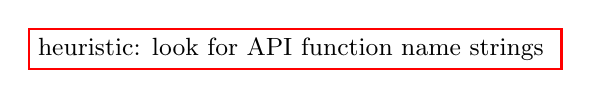
\begin{tikzpicture}
\tikzset{
    annoBox/.style={draw=red,thick,font=\small,align=center},
}
    \node[annoBox] {
        heuristic: look for API function name strings
    };
    \end{tikzpicture}
\end{frame}

\begin{frame}{evading library call checking}
    \begin{itemize}
    \item modify dynamic linking tables
        \begin{itemize}
        \item probably tricky to add new entry
        \end{itemize}
    \item reimplement library call manually
        \begin{itemize}
        \item Windows system calls not well documented, change
        \end{itemize}
    \item \myemph<2>{hide names}
    \end{itemize}
\end{frame}

\begin{frame}{hiding library call names}
    \begin{itemize}
    \item common approach: store \myemph{hash of name}
    \item runtime: read library, scan list of functions for name
    \vspace{.5cm}
    \item bonus: makes analysis harder
    \end{itemize}
\end{frame}




\section{behavior based detection}
\begin{frame}{behavior-based detection}
    \begin{itemize}
    \item things malware does that other programs don't?
    \vspace{.5cm}
    \item<2-> modify system files
    \item<2-> modifying existing executables
    \item<2-> open network connections to lots of random places 
    \item<2-> \ldots
    \vspace{.5cm}
    \item basic idea: run in virtual machine; and/or monitor all programs
    \end{itemize}
\end{frame}


\subsection{instrumenting programs}
\begin{frame}<1>[label=hookingList]{hooking}
    \begin{itemize}
    \item hooking --- getting a `hook' to run on (OS) operations
        \begin{itemize}
        \item e.g. creating new files
        \item e.g. modifying executable files
        \end{itemize}
    \item ideal mechanism: \myemph<2>{OS support}
    \item less ideal mechanism: \myemph<3>{change library loading}
        \begin{itemize}
        \item e.g. replace `open', `fopen', etc. in libraries
        \end{itemize}
    \item less ideal mechanism: \myemph<4>{replace OS exception} (system call) handlers
        \begin{itemize}
        \item very OS version dependent
        \end{itemize} 
    \item less ideal mechanism: \myemph<5>{debugger support}
    \end{itemize}
\end{frame}

\againframe<2>{hookingList}

\begin{frame}
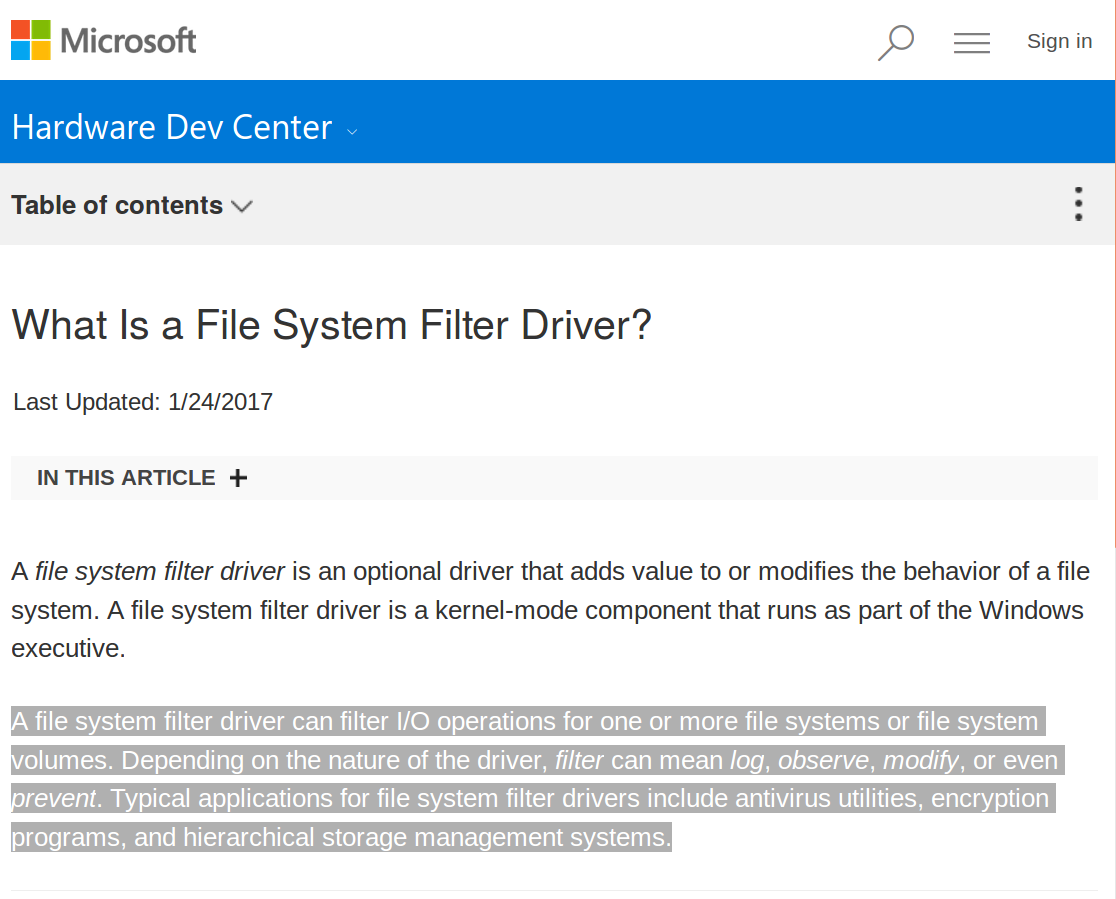
\includegraphics[height=0.9\textheight]{../heur-detect/filter-driver} 
\end{frame}

\begin{frame}{Linux hooking}
\begin{itemize}
\item several possible mechanisms
\item tracepoints, kprobes
    \begin{itemize}
    \item cause hooking functions to run when kernel functions called or return
    \item hooker function can arrange for logging or other action
    \end{itemize}
\item seccomp BPF
    \begin{itemize}
    \item allow hooker to write `program' to examine system calls of selected processes
    \item can deny/change/log those system calls
    \end{itemize}
\end{itemize}
\end{frame}

\begin{frame}{aside Linux eBPF}
    \begin{itemize}
    \item eBPF = extended Berkeley Packet Filters
    \item little programming language originally intended for network filtering
    \item 
    \end{itemize}
\end{frame}

\againframe<3>{hookingList}

\begin{frame}{changing library loading}
\begin{itemize}
    \item e.g. install new library --- or edit loader, but \ldots
    \vspace{.5cm}
    \item not everything uses library functions
    \item what if your wrapper doesn't work exactly the same?
\end{itemize}
\end{frame}

\againframe<4>{hookingList}

\begin{frame}{changing exception call handlers (1)}
    \begin{itemize}
    \item OS data structure tells hardware where program requests go
    \item simpliest mechanism: edit that data structure
       \begin{itemize}
       \item and save a copy of what was there before
       \end{itemize}
    \item point to your code
        \begin{itemize}
        \item and call what was there before after behavior check
        \end{itemize}
    \end{itemize}
\end{frame}



\section{AI heuristic case study: DREBIN}

\begin{frame}{heuristics example: DREBIN paper}
    \begin{itemize}
    \item {\small from 2014 research paper on Android malware: Arp et al, ``DREBIN: Effective and Explainable Detection of Android Malware in Your Pocket''}
    \item primary contribution of paper: big dataset of malware
    \item but tried to detect malware, too\ldots
    \item features from applications (\myemph{without running}):
        \begin{itemize}
        \item hardware requirements
        \item requested permissions
        \item whether it runs in background, with pushed notifications, etc.
        \item what API calls it uses
        \item network addresses
        \end{itemize}
    \item detect \myemph{dynamic code generation} explicitly
    \item statistics (i.e. machine learning) to determine score
    \end{itemize}
\end{frame}

\begin{frame}{heuristics example: DREBIN paper}
    \begin{itemize}
    \item advantage: Android uses Dalvik bytecode (Java-like)
        \begin{itemize}
        \item high-level ``machine code''
        \item much easier/more useful to analyze
        \end{itemize}
    \item accuracy?
        \begin{itemize}
        \item tested on 131k apps, $94$\% of malware, $1$\% false positives
        \item versus best commercial: $96$\%, $<0.3$\% false positives
            \begin{itemize}
            \item (probably has explicit patterns for many known malware samples)
            \end{itemize}
        \end{itemize}
    \item \ldots but
        \begin{itemize}
        \item statistics: training set needs to be typical of malware
        \item cat-and-mouse: what would attackers do in response?
        \end{itemize}
    \end{itemize}
\end{frame}


\subsection{machine learning and adversaries}
\begin{frame}{machine learning and adversaries}
    \begin{itemize}
    \item I don't like most ML-based approaches to malware detection
    \vspace{.5cm}
    \item problem: most machine learning not designed to deal with adversaries
    \item attack: find factors used to ID benign programs
        \begin{itemize}
        \item do all of them as much as possible
        \item inquiry: what might they be in DREBIN case?
        \end{itemize}
    \item attack: provide many malware samples with benign weird behavior
        \begin{itemize}
        \item machine learning uses weird behavior to identify malware
        \item may lower effectiveness on `normal' malware
        \end{itemize}
    \end{itemize}
\end{frame}




\section{backup slides}
\begin{frame}{backup slides}
\end{frame}

\end{document}
